\section{Sets and Relations}

\frame{
{Part 3: Sets and Relations}

\tableofcontents[currentsection,hideallsubsections, firstsection=2, sections={2-4}]
}

\subsection{Sets: Definitions}
\begin{frame}
  \frametitle{Mathematical Set}

  \structure{Mathematical Sets} are useful when talking about proofs.\bigskip
  
  We have already used some sets: \bigskip

  \begin{itemize}
    \item $\mathbb{N}$ -- Set of natural (non negative) numbers;
    \item $\mathbb{Z}$ -- Set of integer numbers;
    \item $\mathbb{R}$ -- Set of real numbers;
  \end{itemize}
\end{frame}

\begin{frame}
  \frametitle{Characteristics of Mathematical Sets}

  \begin{itemize}
    \item  \structure{Sets} can mix different "types" of objects:
    \begin{itemize}
    \item \{7, ``Aranha'', $\pi/2$, TRUE\}
    \end{itemize}\medskip

    \item \structure{Sets} do not have a concept of "order":
    \begin{itemize}
      \item \{7, ``Aranha'', $\pi/2$, TRUE\} is the same as \item \{TRUE, 7, $\pi/2$, ``Aranha''\}
    \end{itemize}\medskip

    \item \structure{Sets} do not contain duplicates:
    \begin{itemize}
    \item \{7, $\pi$\} = \{7, $\pi$, 7\}
    \end{itemize}\medskip

    \item \structure{Sets} can be Infinite: $\mathbb{N}, \mathbb{R}, \ldots$\medskip
    
    \item The empty set: $\varnothing = \{\}$
  \end{itemize}
\end{frame}


\begin{frame}[t]{Set Membership}

  The fundamental property of a set is \structure{membership}, represented by the symbol $\in$.\bigskip

  \begin{columns}
    \column{.5\textwidth}
  Set A = \{7, TRUE, $\pi$\}
  \begin{itemize}
  \item $7 \in A$
  \item 7 is an element of $A$,
  \item 7 is in $A$,
  \item $3 \notin A$
  \end{itemize}\bigskip

  \column{.5\textwidth}
  Set B = \{7, $\mathbb{Z}$, 3\}
  \begin{itemize}
    \item $7 \in B$
    \item $7 \in \mathbb{Z}$
    \item $\mathbb{Z} \in B$
    \item \alert{$1 \notin B$}
  \end{itemize}
\end{columns}\bigskip

Note that membership is \alert{not} recursive!\bigskip

$1$ belongs to the set $\mathbb{Z}$, but $1$ does not belong to the set $B$.
\end{frame}

\begin{frame}[t]{Set Builder Notation}
  We can use \structure{Predicates} to construct sets. The set is composed of all value for which the predicate is true. For example:\bigskip 

  \begin{itemize}
  \item $A ::= \{n \in \mathbb{N} | n \text{ is a prime and } n = 4k + 1 \text{ for } k \in \mathbb{Z} \}$
  \item $B ::= \{x \in \mathbb{R} | x^3 - 3x + 1 > 0\}$
  \item $C ::= \{a^2 | a = b^2, a, b \in \mathbb{N}\}$ 
  \end{itemize}\bigskip

  Please list a few elements of each set. This looks like python's comprehension lists!
\end{frame}

\begin{frame}[t]{Set: Subsets}

  {\larger
  \begin{block}{Subset}
    \begin{itemize}
    \item $A \subset B$ means that every element of A is also an element of B
    \item $A\subset B \equiv \forall x, x\in A \rightarrow x\in B$
    \item $\mathbb{Z} \subset \mathbb{R}, \mathbb{R} \subset \mathbb{C}, \{3\} \subset \{5,3,7\}$
    \end{itemize}
  \end{block}

  \begin{block}{Important!}
    \begin{itemize}
    \item $A \subset A$
    \item Every set contains the empty subset: $\forall X, \varnothing \subset X$
    \end{itemize}
  \end{block}
  }
\end{frame}

\begin{frame}
  \frametitle{Difference between Membership and Subset}

  \begin{columns}[T]
    \column{0.5\textwidth}
    \structure{Membership} ($\in, \notin$) indicates if one member is part of a set. \structure{Subset} ($\subset, \not\subset$) indicates if one set contains the members of other sets.

    \column{0.5\textwidth}
  {\larger
  \begin{itemize}
  \item $3 \in \{3,5,6\}$
  \item $3 \not\subset \{3,5,6\}$
  \end{itemize}
  \bigskip

  \begin{itemize}
  \item $\{3\} \subset \{3,5,6\}$
  \item $\{3\} \notin \{3,5,6\}$
  \end{itemize}
  \bigskip

  \begin{itemize}
    \item \alert{$\{3\} \in \{5, 6, \{3\}\}$}
  \end{itemize}
  }
  \end{columns}
\end{frame}

\begin{frame}[t]{Power Set}
  The \structure{Power Set} of A is a special set composed of ALL subsets of A.

  \begin{equation*}
    POW(A) = \forall x \subset A, x \in POW(A)
  \end{equation*}

  For example: $POW(\{T,F\}) = \{\{T\},\{F\},\{T,F\},\varnothing\}$\vfill
    
  \alert{Check the following}: If a set $A$ is a subset of $B$, then $A$ is a member of POW$(B)$

  \begin{equation*}
    \mathbb{N} \subset \mathbb{R}, \mathbb{N} \notin \mathbb{R}, \mathbb{N} \in POW(\mathbb{R})
  \end{equation*}
\end{frame}


\begin{frame}{Operations on Sets}

  Finally, You should be familiar with the regular operations on sets:
  \bigskip

    \begin{itemize}
    \item Union: $A \cup B \rightarrow x \in A \lor x \in B$\bigskip
    \item Intersection: $A \cap B \rightarrow x \in A \land x \in B$\bigskip
    \item Subtraction: $A - B \rightarrow x \in A \land x \notin B$\bigskip
    \item Complement: $\overline{A} = D - A$, where $D$ is the \structure{domain}\\ (the "everything" set or "parent" set of interest).
    \end{itemize}
\end{frame}

\subsection{Sets and Proofs}

\begin{frame}[t]{Example of proofs using sets (1)}

  \begin{proof}[Prove that the empty set is a subset of every set.]
    Proof by construction:

  \begin{enumerate}

  \item $A \subset B$ means that $\forall x, x \in A \rightarrow x \in B$\bigskip

  \item If $A = \varnothing$ then $x \in A$ is FALSE for $\forall x$, so we can replace ``$\forall x \in A$'' with FALSE in {\bf (1)}\bigskip

\item The statement FALSE $\rightarrow x \in B$ is always TRUE.\\ \hfill (remember that FALSE $\rightarrow X$ is always TRUE)\bigskip

  \item Therefore, $\varnothing \subset B$ is TRUE $\forall B$
  \end{enumerate}
  \end{proof}
\end{frame}


\begin{frame}[t]{Sets and Proofs Example (2)}

  \begin{equation*}
    A \cup (B \cap C) \iff (A \cup B) \cap (A \cup C)
  \end{equation*}

  \begin{proof}[Proof that Union and Intersection are Distributive]
    Proof by sequence of "IFF"s:
    \begin{enumerate}
    \item \structure{$x \in A \cup (B \cap C)$} {\bf iff}
    \item $x \in A \lor x \in (B \cap C)$ {\bf iff} \hfill (definition of union)
    \item $x \in A \lor (x \in B \land x \in C)$ {\bf iff} \hfill
      (definition of intersection)
    \item $(x \in A \lor x \in B) \land (x\in A \lor x \in C)$ {\bf
      iff} \hfill (distributive prop.)
    \item $(x \in A\cup B) \land (x \in A\cup C)$ {\bf iff}\hfill
      (definition of union)
    \item \structure{$x \in (A\cup B)\cap (A\cup C)$}  \hfill
      (defintion of intersection)

    \end{enumerate}
  \end{proof}
\end{frame}

\begin{frame}[t]{Sequences and Sets}
  A \alert{sequence} is another kind of mathematical object. It is similar to a set, but \alert{different in important ways.}\bigskip 

  \begin{itemize}
  \item Sequences are represented by parenthesis: $(1, 2, 1), (T, F)$
  \item Sequences can have repeated elements: $(T, T, T, F, F)$
  \item The order of elements in a sequence is important: $(0, 1) \neq (1, 0)$
  \end{itemize}\bigskip 

  We often see sequences as the products of \structure{multiplication between sets}:\bigskip

  \begin{itemize}
    \item All binary sequences with 3 elements: $\{0,1\}^3 = (0, 0, 0), (0, 0, 1), \ldots (1, 1, 1)$
    \item All pairs of two natural numbers: $\mathbb{N}^2 = (0, 0), (0, 1), (0, 2), (0, 3) \ldots (100, 7) \ldots$
  \end{itemize}
\end{frame}


\subsection{Binary Relations}
\begin{frame}
  \frametitle{Definition of Binary Relations}
  \structure{Binary Relations} define an association of elements from one set (the {\bf domain}) to another set (the {\bf co-domain}). We see (binary) relations in many different situations:\bigskip

  \begin{itemize}
    \item Functions are a special case of binary relations: f(x) = y.
    \begin{itemize}
      \item A function associates the set of inputs with the sets of outputs;
    \end{itemize}\bigskip

    \item Operations such as set membership can be expressed as binary relations.
    \begin{itemize}
      \item For example, the predicate \structure{$P(x): x \text{ is prime}$} defines a binary relation from $\mathbb{N}$ to \{TRUE, FALSE\}
    \end{itemize}\bigskip

    \item "Relational Databases" (for example, SQL) are also based on the idea of binary relations
    \begin{itemize}
      \item Key of X, member of a table, joint key, etc;
    \end{itemize}
    \end{itemize}
\end{frame}

\subsection{Binary Relation Definitons}

\begin{frame}[t]{Example of Binary Relation}
  Relation \structure{$P(x): x \text{ is prime}$}:\bigskip

  \begin{itemize}
  \item Domain: $x \in \mathbb{N}$
  \item Co-Domain: $P(x) \in \{True, False\}$ 
  \item Examples:\\ $P(1) = False$\\ $P(3) = True$\\$P(13) = True$\\$P(20) = False$
  \end{itemize}\bigskip 

  It is common to represent binary relations as a graph between the \structure{domain} and the \structure{co-domain}.


\end{frame}

\begin{frame}[t]{Binary Relations as a Graph}

  \begin{columns}[t]
    \column{0.4\textwidth}
    Let's consider the binary relation {\bf R} from a set of students {\bf (D)} that are registered to a set of courses {\bf (J)}.\bigskip

    \begin{itemize}
    \item \structure{Domain}: Set of students;
    \item \structure{Co-domain}: Set of courses;
    \item \alert{Vertices:} Domain and Co-domain are represented as vertices;
    \item \alert{Edges:} Directed edges from Domain to Co-domain;
    \end{itemize}\bigskip

    \column{0.6\textwidth}

    \begin{center}
      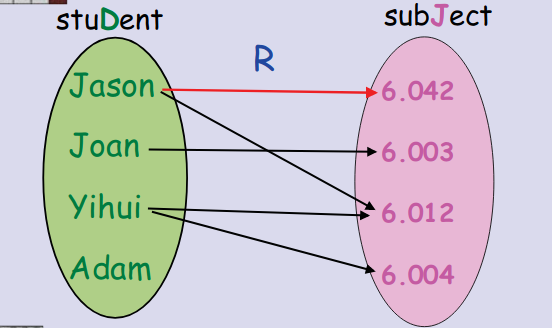
\includegraphics[width=0.6\textwidth]{../img/relations}
    \end{center}\pagenote{Relation Graph Image from MIT OCS}
    Notation to describe the relation:
    \begin{itemize}
    \item $R($Jason$) = \{6.042, 6.012\}$
    \item Jason $R$ 6.042
    \item $R(\{$Jason, Yihui$\}) = \{6.042, 6.012, 6.004\}$
    \end{itemize}
  \end{columns}
\end{frame}


\begin{frame}{Relations and Inverse Relations}

  If we think of a binary relation as a directed graph, the \structure{Inverse Relation} is the relation defined by the same graph when the edges are reversed:\bigskip

  Relation $R$:
  \begin{equation*}
    R(X) ::= {j \in J | \exists d \in X, d R j}
  \end{equation*}

  Reverse Relation $R^{-1}$:
  \begin{equation*}
    R^{-1}(Y) ::= {d \in S | \exists j \in Y, d R j}
  \end{equation*}
  \bigskip

  \begin{columns}
    \column{0.5\textwidth}
    \begin{itemize}
      \item $R(Jason) = \{6.042, 6.012\}$
      \item $R^{-1}(6.012) = \{Jason, Yihui\}$
    \end{itemize}
    \column{0.5\textwidth}
    \begin{center}
      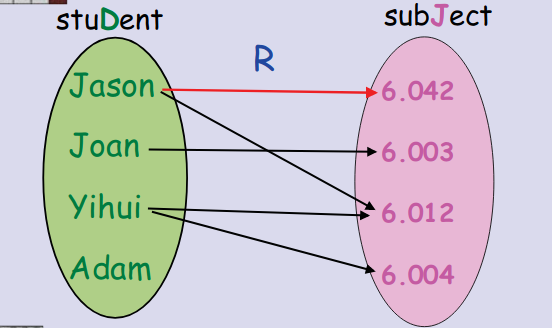
\includegraphics[width=0.6\textwidth]{../img/relations}
    \end{center}
  \end{columns}
\end{frame}

\begin{frame}[t]{Composite Relations}

  \begin{columns}[t]

    \column{0.5\textwidth}
    If we have a relation $V$ from set $P$ to set $D$, and a relation $R$ from set $D$ to set $J$, then we can define a \structure{composite} relation $R\circ V$ from set $P$ to set $J$ (we can also use $R(V)$).\bigskip

    \begin{itemize}
    \item $R(V(X))$ or $(R\circ V)(X)$
    \item $R(V(\text{FTL})) = \{6.003\}$
    \begin{itemize}
      \item professor FTL super{\bf V}ises Joan;\bigskip

      \item Joan is {\bf R}egistered to class 6.003;\bigskip

      \item professor FTL {\bf VR} 6.003 (superregister?)
    \end{itemize}
    \end{itemize}


    \column{0.5\textwidth}
    \begin{center}
      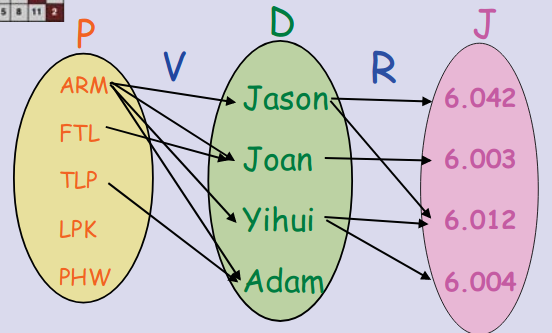
\includegraphics[width=0.8\textwidth]{../img/composite_relation}
    \end{center}

  \end{columns}
\end{frame}


\begin{frame}{Types of Binary Relations}

  We can classify a binary relation based on the number of degrees (arrows) in the relation graph. Imagine a relation $R$ from $X$ to $Y$ (i.e.: $R(X) = Y$)\bigskip

  Classification of $R$ based on $Y$:
  \begin{itemize}
  \item {\bf Surjection}: Every element in $Y$ has $\geq 1$ in-arrows. (Every Y has {\bf one or more} X)
  \item {\bf Injection}: Every element in $Y$ has $\leq 1$ in-arrows. (Every Y has {\bf one or less} X)
  \end{itemize}\smallskip

  Classification of $R$ based on $X$:
  \begin{itemize}
  \item {\bf Total}: Every element in $X$ has $\geq 1$ out arrows. (Every $X$ has {\bf one or more} $Y$)
  \item {\bf Function}: Every element in $X$ has $\leq 1$ out arrows. (Every $X$ has {\bf one or less $Y$})
  \end{itemize}\smallskip

  An important definition:
  \begin{itemize}
  \item {\bf Bijection}: Every element of $X$ has {\bf exactly one} element of $Y$, {\bf and vice versa}.
  \end{itemize}
\end{frame}

\begin{frame}
  \frametitle{Types of Binary Relations: Examples}

    \begin{block}{Example 1: $g: \mathbb{R}\times\mathbb{R} \rightarrow \mathbb{R}, g(x,y) = 1/(x-y)$}
      \begin{itemize}
      \item This is a {\bf function}, because each pair $(x,y)$ has at most one output.
      \item This is not {\bf total}, because not every pair $(x,y)$ has an output: $(x = y)$ has no output.
      \end{itemize}
    \end{block}

    \begin{block}{Example 2: $g_o: \mathbb{R}\times\mathbb{R} - \{x,y|x=y\} \rightarrow \mathbb{R}, g_o(x,y) = 1/(x-y)$}
      \begin{itemize}
      \item $g$ and $g_o$ are similar relations, but defined on different domains.
      \item The domain of $g_o$ removes all $(x,y)$ where $x = y$
      \item Because of this, $g_0$ is {\bf function} (every pair has at most one output) and {\bf total} (every pair has at least one output).
      \end{itemize}

    \end{block}

\end{frame}

% \begin{frame}
%   \frametitle{Size of Finite Sets}
%
%   {\larger
%     We can use the characteristics of relations to estimate the
%     size of sets (domains and co-domains).
%
%     \vfill
%
%     \begin{itemize}
%     \item A bijection B $\rightarrow |A| = |B|$
%     \item A function surjection B $\rightarrow |A| \geq |B|$
%     \item A total injection B $\rightarrow |A| \leq |B|$
%     \end{itemize}
%   }
% \end{frame}
%
% \begin{frame}
%   \frametitle{Set Size Example: Finite power sets and binary strings}
%
%   {\larger
%     What is the size of the Power Set of a \structure{finite} set?
%
%     \vfill
%
%     \begin{itemize}
%     \item Make a bijection between the power set and the binary string
%     \item Calculate the size of a binary string
%     \item Establish equality
%     \end{itemize}
%
%   }
% \end{frame}
